\begin{figure}[!htbp]
\centering
\begin{minipage}[t]{.485\linewidth}
\centering
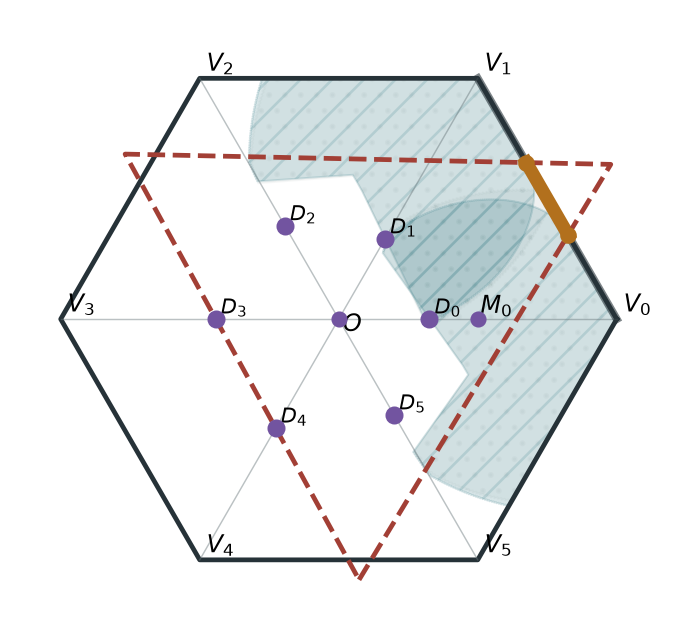
\includegraphics[width=\linewidth]
  {figures/trace_exact_ab/one_gap_n0_vd0.png}
\par\smallskip
\textbf{All \(\Vdzero\).}\par\smallskip
{\footnotesize
\(\begin{gathered}
N_{\rm gap}=1\\
N_+=0\\
(d,t)=(0,0)
\end{gathered}\)}
\end{minipage}\hfill
\begin{minipage}[t]{.485\linewidth}
\centering
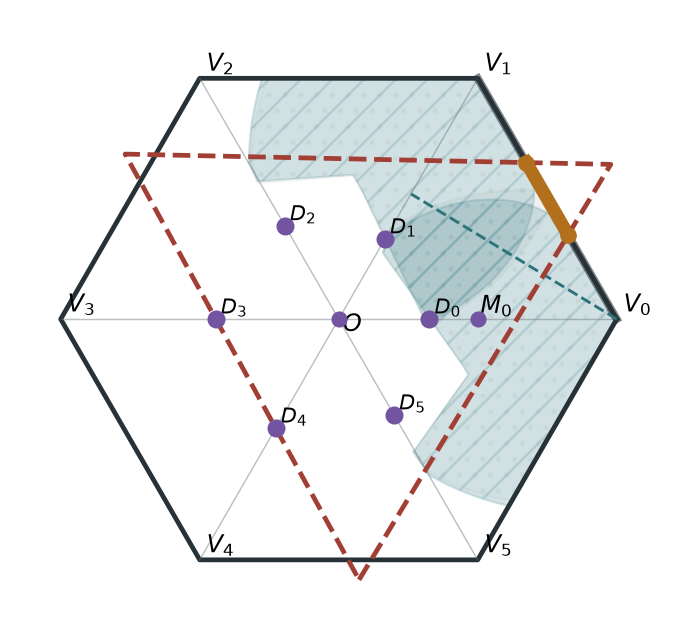
\includegraphics[width=\linewidth]
  {figures/trace_exact_ab/one_t3_n0.png}
\par\smallskip
\textbf{One \(\Tlike\) role.}\par\smallskip
{\footnotesize
\(\begin{gathered}
N_{\rm gap}=1\\
N_+=0\\
(d,t)=(0,1)
\end{gathered}\)}
\end{minipage}

\par\medskip
\begin{minipage}[t]{.485\linewidth}
\centering
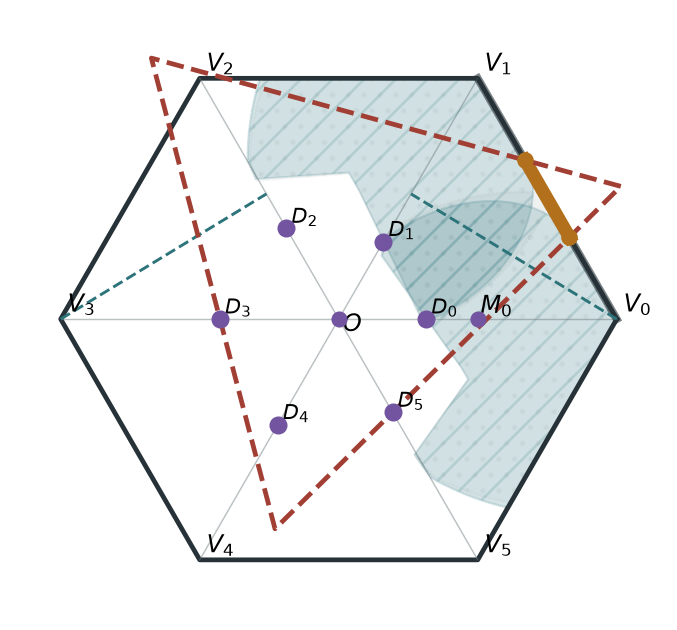
\includegraphics[width=\linewidth]
  {figures/trace_exact_ab/two_t3_n0.png}
\par\smallskip
\textbf{Two \(\Tlike\) roles.}\par\smallskip
{\footnotesize
\(\begin{gathered}
N_{\rm gap}=1\\
N_+=0\\
(d,t)=(0,2)
\end{gathered}\)}
\end{minipage}
\caption{Case A: sampled complementary-gap data.}
\label{fig:finite-enclosure-case-a-examples}
\end{figure}
